\documentclass{scrreprt}
\usepackage{standalone}
\usepackage{caption}
\usepackage{subcaption}
\usepackage{graphbox} % 1120
\usepackage{chez}

\title{Vector Calculus -- Honors}
\author{Neo Wang\\ Lecturer: William Bekcner}
\date{Last Updated: \today}

\begin{document}
\maketitle


\chapter{Chapter 1}

\section{Lecture 1--August 22, 2022}

Riemann integrals deal with functions that are basically continuous.
You should use the notation $(x, y, z)$ or $x\hat{i} + y\hat{j} + z\hat{k}$

There are several coordinates: Cartesian, cylindrical, and spherical.

Spherical coordinates are given by $(r, \theta, \phi)$

\begin{example}
	Let $f$ by a continuous functions. Suppose $f(x,y,z)=g(\sqrt{x^2+y^2+z^2})$.

	Let 1. $f(x)=g(\sqrt{x^2+y^2+z^2})$
	and 2. $f(x, y, z) = h_1(\abs{x})h_2(\abs{y})+h_3(\abs{z})$

	how many such functions satisfy this?
\end{example}

\begin{definition}
	Some useful integrals
	\begin{itemize}
		\item Continuous: $dxdydz$
		\item Cylindrical: $rdrd\theta$
		\item Spherical: $r^2\sin\theta drd\theta d\phi$
	\end{itemize}
\end{definition}

\begin{definition}[Vectors]
	Cross product: $\vec{x}\wedge \vec{y} = -\hat{y} \wedge \hat{x}$ is a vector operation

	Dot product: $\vec{x}\cdot \vec{y} = \sum x_i y_i$ is a scalar operation
\end{definition}

\section{Lecture 2--August 23, 2022}

\begin{definition}[Coordinate Systems]

$\vec{v}=(x,y,z)\rightarrow \vec{x}=(x_1,x_2,x_3)$

Sometimes will not include $\vec{}$ symbol--we want to think more abstractly in order to build to higher concepts.
Spherical coordinates: $(r,\theta,\phi)$, and $\theta$ is always the polar angle (from $z$-axis).

Orientation is the order of $(x, y, z)$ which comes into play with \boxed{\text{change of variables.}}

\end{definition}

\begin{remark}[Property of the determinant]
	The determinant is always $+$ or $-$
\end{remark}

There are several volume form differentials:
\[
	dxdydz = r^2dr\sin \theta d\theta d\phi
\]
and note that $\sin \theta$ is always positive

\begin{remark}[Normal model]
	Normal distribution pdf: \[p(x)=\frac{1}{\sqrt{2\pi}}e^{-\frac{1}{2}x^2}\]
	With $\mu=0$ and $\sigma=0$
	The error function is the simplest example of a function that is ``not integrable in elementary terms''

	\begin{align*}
		2 \int_0^\infty e^{-x^2}dx &= \sqrt{\pi}
	\end{align*}

	There are connections with physics i.e. the uncertainty principle and the quantum mechanics harmonic oscillator.

	\begin{align*}
		A &= \int_{-\infty}^{\infty} e^{-x^2}dx \\
		A^2 &= \int_{-\infty}^{\infty} \int_{-\infty}^{\infty} e^{-x^2 - y^2} dydx \\
			&= \int_{0}^{2\pi}\int_{0}^{\infty} e^{-r^2}rdrd\theta \\
			&= \frac{1}{2}\int_{0}^{2\pi} \int_{\infty}^{0} e^{-u}dud\theta \\
			&= \frac{1}{2}\int_{0}^{2\pi} 1 d\theta \\
			&= \pi \\
			\Aboxed{A &= \sqrt{\pi}}
	\end{align*}
\end{remark}

Differentials tell you how to compute an integral.

\begin{enumerate}
	\item The integral is linear (also the derivative)
	\[
		\int(af+bg)dm=a\int fdm + b\int gdm
	\]
	\item For a non-negative function $f(x)\geq 0$ any way that you can calculate a
	finite value for the integral gives you the ``correct answer.''
	\item Dilation: \[
		\int_0^\infty f(ax)dx=\frac{1}{a}\int_0^\infty f(x)dx
	\]
\end{enumerate}

\begin{remark}[For proving estimates for the dot or scalar product]

Estimate: $\abs{x\cdot y}=\abs{\sum x_i y_i}\leq||\vec{x}||||\vec{y}||, x =(x_1,x_2,x_3), y=(y_1,y_2,y_3)$ 

3 simple arguments:
\begin{enumerate}
	\item Euclidian geometry
	\item Arithmetic
	\item Adding a variable $\leftarrow$ the best way and expands view to another parameter
\end{enumerate}
\end{remark}
Properties of vectors:
vector products (may be a scalar $\vec{x}\cdot \vec{y}$ or a vector $\vec{x}\wedge \vec{y}$) and representation of data in terms of partial derivatives.

\section{Discussion--August 24, 2022}

Vectors are a directed line segment. A vector in $n$-dimensional space is an
ordered tuple of $n$ real numbers. A vector is denoted $\vec{v}=(a_1,\ldots, a_n), a_i \in \mathbb{R}$

The basic operations:

\begin{itemize}
	\item Addition of vectors: $\vec{v}+\vec{w}=(a_1+b_1,\ldots, a_n+b_n)$
	\item Multiplication by scalar: $c\vec{v}=(ca_1,\ldots, ca_n)$
\end{itemize}

Properties:

\begin{itemize}
	\item $\forall \vec{u}\in \mathbb{R}^n \langle \vec{u}, \vec{u}\rangle \geq 0$
	\item $\langle u, v \rangle = \langle v, u \rangle$
	\item Dot product is linear: \[
		c(u\cdot v) = (cu)\cdot v = u\cdot (cv)
	\]
\end{itemize}

\section{Lecture 3--August 25, 2022}

How to think about data: strings, words, ``columns'', rectangular arrays.

We can think of strings as slots: $(x_1, x_2, x_3, \ldots, x_n)$

Structures of organization may give insightful information on how to extra information

\begin{definition}[Triangle Inequality]
	The length of any side is less than the sum of the lengths of the other two sides.
\end{definition}

More abstract setting--use ``norm.'' Vectors: objects that we can add or subtract scalar mltiples--scalars.

Length--norm: $\abs{\vec{v}}=\sqrt{\langle \vec{v}, \vec{v}\rangle}$

\begin{definition}[Homogenous]
	A real-valued function $h(x)$ is homogenous of degree $\lambda$
	if $h(\lambda x)=\delta^\lambda h(x)$ where $\lambda \in \mathbb{R}$

	The differential $r^2drsin\theta d\theta d\phi$ is homogenous of degree $3$.

	This defines a vector space.
\end{definition}

\begin{remark}[Most important property from linear algebra]
	Suppose you have a finite collection of vectors which you want to be \fbox{linearly independent.}
	Then you can find a basis for the space spanned by the vectors. Then:
	\[
		c_1u_1 + c_2u_2 + \ldots + c_nu_n = 0 \Leftrightarrow c_1=c_2=\ldots=c_n=0
	\]

	in $\mathbb{R}^3$, the unit vectors $\vec{i}, \vec{j}, \vec{k}$ are linearly independent.
	Any vector expression written in terms of these vectors is unique. The only way
	for us to get the zero vector is if all the coefficients are zero.

\end{remark}

A vector space with a norm is called a ``normed vector space.''

\begin{example}[Normed vector space]
	Consider the set of continuous functions defined on the unit square--with scalars
	as real numbers, they are vector space. Restrict to all such functions that are
	square integrable on the unit square:

	\[
		\int_0^1\int_0^1|f(x,y)|^2dx dy < \infty
	\]

	if this is true then we can create a norm on this space by setting 

	\[
		||f|| = \sqrt{\int_0^1\int_0^1|f(x,y)|^2dxdy}
	\]

	\[
		||f||_2 = \int_0^1\int_0^1|f(x,y)|dxdy
	\]

	Then we have informally said that $f$ is Lebesgue integrable.
\end{example}

\begin{remark}
The function is defined for a domain and the function takes various values. What do you want to
partition? You want to partition the range and you can estimate the function in order to get the
Lebesgue integral. We can look at this fundamental difference via the diagram (Lebesgue on bottom):

% lesbesgue diagram
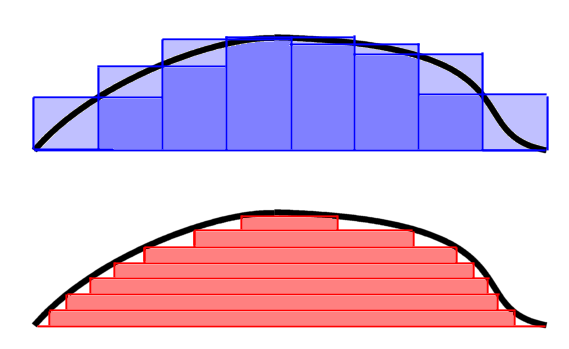
\includegraphics[width=300px]{figures/2022-08-25-11-47-29.png}
\end{remark}

\begin{fact}[Dot Product]
	$\vec{x}\cdot \vec{x} = \abs{\vec{x}}^2$
\end{fact}

\begin{theorem}[Cauchy Schwartz Inequality]
	With respect to length--to show that for two vectors $\vec{x} = (x_1, x_2, x_3)$ and $\vec{y} = (y_1, y_2, y_3)$ then 
	\[
		\abs{\vec{x}\cdot \vec{y}} \leq |\vec{x}| |\vec{y}|.
	\]

	same argument will work for abstract vector spaces with norm and scalar product.

	Multiple proofs: Euclidean geometry, arithmetic, to see the role of length. But proof should capture the spirit of calculating length.

	\begin{proof}
		We will add a parameter $\lambda$ 

		\[
			|\vec{x} - \lambda \vec{y}|
		\]

		Remember that lengths and norms have corners. These are not smooth.
		For example $f(x=|x|)$ is not smooth at $x=0$. You would like to smooth it
		out to something like $g(x)=x^2$. Therefore, square the expression to remove the ``corners.''

		Assume that $\vec{x}$ and $\vec{y}$ are non-zero. Otherwise nothing to show.

		\begin{align*}
			0 \leq |\vec{x}-\lambda \vec{y}|^2 &= \vec{x}\cdot \vec{x} + \lambda^2\vec{y}\cdot \vec{y} - 2\lambda\vec{x}\cdot \vec{y} \\ &= \abs{\vec{x}}^2 + \lambda^2\abs{\vec{y}}^2 - 2\lambda\vec{x}\cdot \vec{y} \\
			&= |y|^2 + \brackets{\lambda^2-2B\lambda+C} \\
			&= \lambda^2 - 2B\lambda + C
		\end{align*}

		If we complete the square we get $\lambda^2-2B\lambda + B^2 + C - B^2\geq 0$

		\[
			(\lambda - B)^2 + C - B^2 \geq 0 \implies \boxed{C-B^2\geq 0}
		\]

		\[
			C = \frac{|x|^2}{|y|^2}, B = \frac{x\cdot y}{|y|^2}
		\]

		Expanding this, we get the Cauchy Schwartz inequality.
	\end{proof}
\end{theorem}

We want to extend length of vectors to norms, but also the dot product to scalar products.

\begin{itemize}
	\item $\vec{x}\cdot \vec{y}\rightarrow \angles{x, y}$ (scalar product)
	\item $\angles{x,y}=\angles{y,x}$ symmetry
	\item $\angles{x,\alpha y + \beta z} = \alpha\angles{x, y} + \beta \angles{x, z}$ 
	\item $\angles{x,x} \geq 0$ (positive definite)
	\item $\angles{x,x} = \norm{x}^2$
\end{itemize}



\end{document}